\documentclass[a4paper]{article}

\usepackage[english]{babel}
\usepackage[utf8]{inputenc}
\usepackage{amsmath}
\usepackage{graphicx}
\usepackage[colorinlistoftodos]{todonotes}


\usepackage[algo2e]{algorithm2e}
\usepackage{algorithmic}  
\usepackage{algorithm}
\usepackage{comment}
\title{Joint Modeling of Content-Partitioned Multinetwork Embeddings (CPME) and Point Process Approach}
\author{Bomin Kim}

\begin{document}
\maketitle

\begin{abstract}
Your abstract.
\end{abstract}

\section{Ideas}
Current CPME model does not involve any of temporal component, which plays a key role in email interactions. Intuitively, past interaction behaviors significantly influence future ones; for example, if an actor $i$ sent an email to actor $j$, then $j$ is highly likely to send an email back to $i$ as a response (i.e. reciprocity). Moreover, the recency and frequency of past interactions can also be considered to effectively predict future interactions. Thus, as an exploratory data analysis, point process model for directional interaction is applied to the North Carolina email data. Starting from the existing framework focused on the analysis of content-partitioned subnetworks, I would suggest an extended approach to analyze the data using the timestamps in the email, aiming to develop a joint dynamic or longitudinal model of text-valued ties.\\ \newline
 CPME model is a Bayesian framework using two well-known methods: Latent Dirichlet Allocation (LDA) and Latent Space Model (LSM). Basically, existence of edge depends on topic assignment t (LDA) and its corresponding interaction pattern c. Each topic t=1,…,T has one interaction pattern c=1,…,C, and each interaction pattern posits unique latent space (LSM), thus generating $A\times A$ matrix of probabilities $P^{(c)}$ that a message author
a will include recipient $r$ on the message, given that it is about
a topic in cluster $c$.  Incorporating point process approach, now assume that under each interaction pattern, we have $A\times A$ matrix of stochastic intensities $\lambda^{(c)}(t)$ which depend on the history of interaction between the sender and receiver. 
\newpage
\section{CPME + Point Process Model}
Before we build up the ultimate joint model of LDA, LSM, and point process approach, we first start with simpler model which combines LDA and point process approach.
\subsection{General framework}
In this section, we introduce multiplicative Cox regression model for the edge formation process in a longitudinal communication network. For concreteness, we frame our discussion of this model in terms of email data, although it is generally applicable to any similarly-structured communication data.\\ \newline A single email, indexed by d, is represented by a set of tokens $w^{(d)} = \{w^{(d)}_n \}_{n=1}^{N^{(d)}}$ that comprise the
text of that email, an integer $a^{(d)} \in \{1,...,A\}$ indicating the identity of that email’s author, and an integer $t^{(d)} \in [0, T]$ indicating the (unix time-based) timestamp of that email. \\ \newline
As in LDA, each email, indexed by d, has a discrete distribution over topics $\theta^{(d)}$. A Dirichlet prior
with concentration parameter $\alpha$ is placed (i.e. $\theta^{(d)}\sim \mbox{Dir}(\alpha, m)$). Then, a “topic” t is characterized by a discrete distribution over $V$ word types with probability vector $\phi^{(t)}$. A symmetric Dirichlet prior with concentration parameter $\beta$ is placed (i.e. $\phi^{(t)} \sim \mbox{Dir}(\beta, n)$). Now, each topic t is associated with one ``interaction pattern" among C different types, which is assigned by $l_t \sim \mbox{Unif}(1, C)$. \\ \newline
To capture the relationship between the interaction patterns expressed in an email and that email’s recipients, topics that share $C$ are associated with an $A\times A$ matrix of $N^{(c)}_{ar}(t)$, a counting process denoting the number of edges (emails) from actor $a$ to actor $r$ up to time $t$. \textcolor{red}{NOTE: We use the partition $C$ since we expect that some topics/interaction patterns have little variation among the pairs of actors (e.g. broadcasting), while some have large variation (e.g. meeting scheduling, personal affairs).} Combining the individual counting processes of all potential edges,  $\mathbf{N}^{(c)}(t)$ is the multivariate counting process with $\mathbf{N}^{(c)}(t)=(N^{(c)}_{ar}(t): a, r \in {1, ..., A}, a \neq r)$. Here we make no assumption about the independence of individual edge counting process. As in Vu et al. (2011b), we model the multivariate counting process via Doob-Meyer decomposition:
\begin{equation}
\mathbf{N}^{(c)}(t)=\int_0^t\boldsymbol{\lambda}^{(c)}(s)ds + \mathbf{M}(t)
\end{equation}
where essentially $\boldsymbol{\lambda}^{(c)}(t)$ and $\mathbf{M}(t)$ may be viewed as the (deterministic) signal and (martingale) noise, respectively.\\ \newline
Following the multiplicative Cox model of the intensity process $\boldsymbol{\lambda}^{(c)}(t)$ given $\boldsymbol{H}^{(c)}_{t-}$, the entire past of the network related to $C$ up to but not including time $t$, we consider for each potential directed edge $(a, r)$ the intensity forms:
\begin{equation}
 \lambda^{(c)}_{ar}(t|\boldsymbol{H}^{(c)}_{t-})=\lambda^{(c)}_0(t)\cdot \mbox{exp}(\beta^{(c)T}x^{(c)}(a, r, t))\cdot 1\{r \in \mathcal{A}^{(c)}_{(a, t)}\}
\end{equation}
where $\lambda_0^{(c)}(t)$ is the baseline hazards for the interaction pattern $C$, $\beta^{(c)}$ is an unknown vector of coefficients in $\boldsymbol{R}^{p}$, $x^{(c)}(a, r, t)$ is a vector of $p$ statistics for directed edge $(a, r)$ constructed based on
$\boldsymbol{H}^{(c)}_{t-}$ (examples of these statistics are given in the next section), and $\mathcal{A}^{(c)}_{(a, t)}$ is the predictable receiver set of sender $a$ at time $t$ within all actors $A^{(c)}$. \textcolor{red}{NOTE: We assume that all possible actor set $A^{(c)}$ varies depending on the interaction pattern (e.g. confidential communication do not move outside of certain actors) }
\subsection{Dynamic covariates to measure network effects}
The network statistics $x^{(c)}(a, r, t)$ of equations (2), corresponding to the ordered pair $(a, r)$, can be time-invariant (such as gender) or time-dependent (such as the number of two-paths from $a$ to $r$ just before time $t$). Since time-invariant covariates can be easily specified in various manners (e. g. homophily or group-level effects), here we only consider specification of dynamic covariates.\\ \newline
Following Perry and Wolfe (2013), we use 6 effects as components of $x^{(c)}(a, r, t)$. The first two behaviors (send and receive) are dyadic, involving exactly two actors,
while the last four (2-send, 2-receive, sibling, and cosibling) are triadic, involving exactly three actors. However, different from Perry and Wolfe (2013), we define the effects not based on finite sub-interval, which require large number of dimention. Instead, we create single statistic for each effect by incorporating the recency of event into the statistic itself. Moreover, we take the interaction pattern $C$ into account as well, based on the topic-token-interaction pattern assignment from LDA. \\ \newline 
1. $\textbf{send}^{(c)}(a, r, t)=\sum\limits_{d: t_d<t} \frac{\bar N^{(c|d)}}{\bar N^{(d)}}\cdot I\{a\rightarrow r\}\cdot g(t-t_d)$\\
2. $\textbf{receive}^{(c)}(a, r, t)=\sum\limits_{d: t_d<t} \frac{\bar N^{(c|d)}}{\bar N^{(d)}}\cdot I\{r\rightarrow a\}\cdot g(t-t_d)$\\
3. $\textbf{2-send}^{(c)}(a, r, t)=\sum\limits_{h \neq a, r}\Large(\sum\limits_{d: t_d<t} \frac{\bar N^{(c|d)}}{\bar N^{(d)}}\cdot I\{a\rightarrow h\}\cdot g(t-t_d)\Large)\Large(\sum\limits_{d: t_d<t} \frac{\bar N^{(c|d)}}{\bar N^{(d)}}\cdot I\{h\rightarrow r\}\cdot g(t-t_d)\Large)$\\
4. $\textbf{2-receive}^{(c)}(a, r, t)=\sum\limits_{h \neq a, r}\Large(\sum\limits_{d: t_d<t} \frac{\bar N^{(c|d)}}{\bar N^{(d)}}\cdot I\{h\rightarrow a\}\cdot g(t-t_d)\Large)\Large(\sum\limits_{d: t_d<t} \frac{\bar N^{(c|d)}}{\bar N^{(d)}}\cdot I\{r\rightarrow h\}\cdot g(t-t_d)\Large)$\\
5. $\textbf{sibling}^{(c)}(a, r, t)=\sum\limits_{h \neq a, r}\Large(\sum\limits_{d: t_d<t} \frac{\bar N^{(c|d)}}{\bar N^{(d)}}\cdot I\{h\rightarrow a\}\cdot g(t-t_d)\Large)\Large(\sum\limits_{d: t_d<t} \frac{\bar N^{(c|d)}}{\bar N^{(d)}}\cdot I\{h\rightarrow r\}\cdot g(t-t_d)\Large)$\\
6. $\textbf{cosibling}^{(c)}(a, r, t)=\sum\limits_{h \neq a, r}\Large(\sum\limits_{d: t_d<t} \frac{\bar N^{(c|d)}}{\bar N^{(d)}}\cdot I\{a\rightarrow h\}\cdot g(t-t_d)\Large)\Large(\sum\limits_{d: t_d<t} \frac{\bar N^{(c|d)}}{\bar N^{(d)}}\cdot I\{r\rightarrow h\}\cdot g(t-t_d)\Large)$\\\newline
Here, $g(t-t_d)$ reflects the difference between current time $t$ and the timestamp of previous email $t_d$, thus measuring the recency. Inspired by the self-exciting Hawkes process, which is often used to model the temporal effect of email data, we can take the exponential kernel $g(t-t_d)=we^{-w(t-t_d)}$ where $w$ is the parameter of speed at
which sender replies to emails, with larger values indicating faster response times. Indeed, $w^{-1}$ is the expected number of hours it takes to reply to a typical email. \textcolor{red}{NOTE: First, we can let $w$ to be hyperparameter to be specified (since $\beta$ will be adjusted to the scale of $w$). However, later we can try to estimate it via Bayesian approach, or even consider sender-specific $w_a$ or pair-specific $w_{ar}$ and estimate them.}
\subsection{Inference}
Assuming each interaction has a single receiver (no multicast), we model the stochastic intensity of the multivariate counting process $N$ as \begin{equation}\lambda_t(i,j)=\bar\lambda_t(i)\cdot \mbox{exp}\{\beta^Tx_t(i, j)\}\cdot 1\{j \in \mathcal{J}_t(i)\},
\end{equation} 
where $\beta$ is an unknown vector of coefficients in $\boldsymbol{R}^{p}$. After treating the baseline rate $\bar\lambda_t(i)$ as a nuisance parameter, estimation for $\beta$ proceeds by maximizing the so-called partial likelihood of \cite{cox1992regression}: 
\begin{equation}
PL_t(\beta)=\prod_{t_m\leq t} \frac{\mbox{exp}(\beta^Tx_{t_m}(i_m, j_m))}{\sum_{j\in \mathcal{J}_{t_m}(i_m)} \mbox{exp}(\beta^Tx_{t_m}(i_m, j))},
\end{equation}
where $t_m$, $i_m$, and $j_m$ are the time, sender, and receiver
of the $m$th event.
Further, we can estimate the coefficient vector $\beta$ using the log-partial likelihood at time $t$:
\begin{equation}
\mbox{log}PL_t(\beta)=\sum_{t_m\leq t} \Big\{\beta^Tx_{t_m}(i_m, j_m)-\mbox{log}\big[\sum_{j\in \mathcal{J}_{t_m}(i_m)} \mbox{exp}\{\beta^Tx_{t_m}(i_m, j)\}\big]\Big\}.
\end{equation}
The function $\mbox{log}PL_t(\cdot)$ is concave, so it can be maximized using the first two derivatives, the gradient $U_t(\beta)=\bigtriangledown[\mbox{log}PL_t(\beta)]$ and negative Hessian $I_t(\beta)=-\bigtriangledown^2[\mbox{log}PL_t(\beta)]$ via the Newton-Raphson algorithm. See \cite{PerryWolfe2012} for the details.\\\\
The model can be extended for interactions that possibly involve a single sender and multiple receivers such as emails, which we call a multicast interaction. Let the tuple $(t, i, J)$ indicate that at time $t$, sender $i$ interacted with receiver set $J$. In addition, let $|J|$ denote the cardinality of the receiver set $J$. Then, we can write the modified version of (3) and (5) as below:
\begin{equation}\lambda_t(i,J)=\bar\lambda_t(i; |J|)\cdot \mbox{exp}\{\sum_{j\in J}\beta_0^Tx_t(i, j)\}\cdot\prod_{j\in J} 1\{j \in \mathcal{J}_t(i)\},
\end{equation}
\begin{equation}
\mbox{log}PL_t(\beta)=\sum_{t_m\leq t} \Big\{\sum_{j\in J_m}\beta^Tx_{t_m}(i_m, j)-\mbox{log}\big[\sum_{\substack{j\subseteq \mathcal{J}_{t_m}(i_m)\\|J|=|J_m|}}\mbox{exp}\{\sum_{j\in  J}\beta^Tx_{t_m}(i_m, j)\}\big]\Big\}.
\end{equation}
Fitting the model above is quite complicated due to the double sums. Thus, instead of using the multicast model, we can use the alternative, the approximate partial loglikelihood, which is obtained by treating the multicast interaction as multiple pairwise interactions. For instance, an email with the tuple $(t, i, J=(j_1, j_2))$ is treated as two separate emails $(t, i, j_1)$ and $(t, i, j_2)$. Under this transformation, the obtained approximate partial loglikelihood is:\begin{equation}
\mbox{log}\widetilde{PL}_t(\beta)=\sum_{t_m\leq t} \Big\{\sum_{j\in J_m}\beta^Tx_{t_m}(i_m, j)-|J_m|\mbox{log}\big[\sum_{j\subseteq \mathcal{J}_{t_m}(i_m)}\mbox{exp}\{\beta^Tx_{t_m}(i_m, j)\}\big]\Big\}
\end{equation}
and $\mbox{log}PL_t(\beta)\approx \mbox{log}\widetilde{PL}_t(\beta)$. To fit the model in a simpler way, we use (8) when estimating the coefficitients $\beta$. For implementation and simulation processes in detail, see \cite{PerryWolfe2012}.  This framework can be viewed as one version of relational event model \cite{Butts2008}, accounting for repeated directed actions and multicast inteactions. Therefore, the coefficients measuring the common effects such as homophily or transitivity can be interpreted in the same context as in \cite{Butts2008}.
\begin{comment}
\subsection{Generative process (From Mattew Denny)}
First we generate the global (corpus-wide) variables. There are two main sets of global variables: those that describe the
topics people talk about and those that describe how people interact (interaction patterns). These variables are linked by a
third set of variables that associate each topic with the pattern that best describes how people interact when talking about
that topic. There are T topics. Each topic $\phi^{(t)}$ is a discrete distribution over V word types \textbf{[See Algorithm 1].} \\ \newline
There are C
interaction patterns. \\ \newline \textcolor{red}{1) Univariate Hawkes approach:} Each interaction pattern consists of a A-dimensional vector of stochastic intensity $\lambda^{(c)}(t)$ that model the rate at which each sender $a$ sends email at time $t$ given all messages received by $a$ at times
$r_k^{a}< t$ ($r_k^{a}$ is the timestamp of $k^{th}$ email received by $a$)  \textbf{[See Algorithm 2].}  \\ \newline
 \textcolor{red}{2) Multivariate Hawkes approach:} Each interaction pattern consists of a A$\times$A matrix of stochastic intensity $\lambda^{(c)}(t)$ that model the rate at which each sender $a$ sends email to actor $r$ at time $t$ given all messages received by $a$ from $r$ at times
 	$r_k^{ar}< t$ ($r_k^{ar}$ is the timestamp of $k^{th}$ email received by $a$ from $r$)  \textbf{[See Algorithm 3].}  \\\newline  (Later goal: We also associate each sender–recipient pair with an observed P-dimensional
vector of covariates $x^{(ar)}$; however, we assume that our generative process is ocnditioned on these covariates.)  The topics and interaction patterns are tied together via a set of T categorical variables (one per topic). These variables
associate each topic with a single interaction pattern \textbf{[See Algorithm 4].} Then, we generate the local variables. There are D
emails. We assume that each email’s sender $a^{(d)}\in [A]$, timestamp $t^{(d)} \in [0, T]$, and length $N^{(d)} \in N_0$ are observed; we do not generate these variables  \textbf{[See Algorithm 5].}
 \begin{algorithm}[H]
 	\SetAlgoLined
	\caption{Topic Word Dstributions}
	\For{t=1 to T}{
		draw $\phi^{(t)}$ $\sim$ Dir($\beta, \bf n$)
}
\end{algorithm}
\begin{algorithm}[H]
	\SetAlgoLined
	\caption{Interaction Patterns using univariate Hawkes Process}
	\For{c=1 to C}{
		\For{a=1 to A}{ 
			set $\lambda_a^{(c)}(t)=\mu_{a}+\theta_{a}\sum\limits_{{r}^{a}_{k}< t} g_a(t-{r}^{a}_{k}) \quad (=\mu_{a}+\theta_{a}\sum\limits_{{r}^{a}_{k}< t}w_{a} e^{-w_a(t-{r}^{a}_{k})})$	}} 
		Note: In the context of e-mails, the background rate $\mu_a$ can be interpreted as that rate at which actor a sends email that are not replies to emails received from other actors. In other words, $\mu_a$ is the baseline rate at which a initiates new email threads. Each message received by actor a at time $r_k^{a}$ elevates the overall rate of sending emails at time $t >r_k^{a}$, through the triggering function, which is assumed to be exponential. $\theta_a$ can be interpreted as the reply rate for actor a, since it is the total expected number of replies, on average, sent by actor a per email received from another actor in the network. The speed at which actor a replies to emails is governed by the parameter $w_a$, with larger values of $w_a$ indicating faster response times for actor a. Indeed, ${w_a}^{-1}$ is the expected number of hours it takes for actor a to reply to a typical email. 
\end{algorithm}
\begin{algorithm}[H]
		\SetAlgoLined
	\caption{Interaction Patterns using multidimensional Hawkes Process} \For{c=1 to C}{ \For{a=1 to A}{	set $\lambda_a^{(c)}(t)$ as the A-dimensional vector of rates defined by a point process $N_t^a$.\\ \For{r=1 to A}{$\lambda_{ar}^{(c)}(t)=\mu_{ar}+\theta_{ar}\sum\limits_{r_k^{ar}< t}g_{ar}(t-r_k^{ar}) (=\mu_{ar}+\theta_{ar}\sum\limits_{r_k^{ar}< t}w_{ar} e^{-w_a(t-r_k^{ar})})$	}}}
	Note: In the context of e-mails, the background rate $\mu_{ar}$ can be interpreted as that rate at which actor $a$ sends email that are not replies to emails received from actor r. In other words, $\mu_{ar}$ is the baseline rate at which a initiates new email threads to r. Each message received by actor a from actor r at time $r_k^{ar}$ elevates the overall rate of sending emails at time $t >r_k^{ar}$, through the triggering function, which is assumed to be exponential. $\theta_{ar}$ can be interpreted as the reply rate for actor a to actor r, since it is the total expected number of replies, on average, sent by actor a per email received from actor r in the network. The speed at which actor a replies to actor r is governed by the parameter $w_{ar}$, with larger values of $w_{ar}$ indicating faster response times for actor a to actor r. Indeed, ${w_{ar}}^{-1}$ is the expected number of hours it takes for actor a to reply to actor r a typical email.	
\end{algorithm}
\begin{algorithm}[H]
		\SetAlgoLined
	\caption{Topic-Interaction Pattern Assginments}
	\For{t=1 to T}{
		draw $l_t$ $\sim$ Unif(1, C)
	}
\end{algorithm}
\begin{algorithm}[H]
	\SetAlgoLined
	\caption{Topic-Interaction Pattern Assginments}
	\For{t=1 to T}{
		draw $l_t$ $\sim$ Unif(1, C)
	}
\end{algorithm}
\end{comment}
\section{Preliminary Analysis}
Hurricane Sandy was the most destructive hurricane in 2012, which hit North Carolina on late October (October 28, Governor Bev Perdue declared a state of emergency in 24 western counties due to snow and strong winds). In our dataset, there are three counties which cover the date of Hurricane Sandy (October 22, 2012 – November 2, 2012), so we focus on the three counties, since the timestamp of email in this case is much more important than usual case without any disastrous event.
\subsection{Dare County}
\footnotesize
\begin{table}[ht]
	\centering
	\begin{tabular}{ |c|ccc|c| } 
		\hline 
		\textbf{Period} &\textbf{Before Sandy} & \textbf{During Sandy} & \textbf{After Sandy} & \textbf{Overall} \\ 	\hline
			\textbf{\# emails}& 1933 & 1563 & 1467 & 4963 \\ 
		\hline
	\end{tabular}
	\caption{ Summary of Dare county email data based on time period}
	\label{table:nullDare2}
\end{table}
\normalsize
Before Sandy ranges from 2012-09-01 to 2012-10-21 (7 weeks), During Sandy ranges from 2012-10-22 to 2012-11-02 (2 weeks), and After Sandy ranges from 2012-11-03 to 2012-11-30 (4 weeks).
\footnotesize
\begin{figure}[ht]
	\centering
	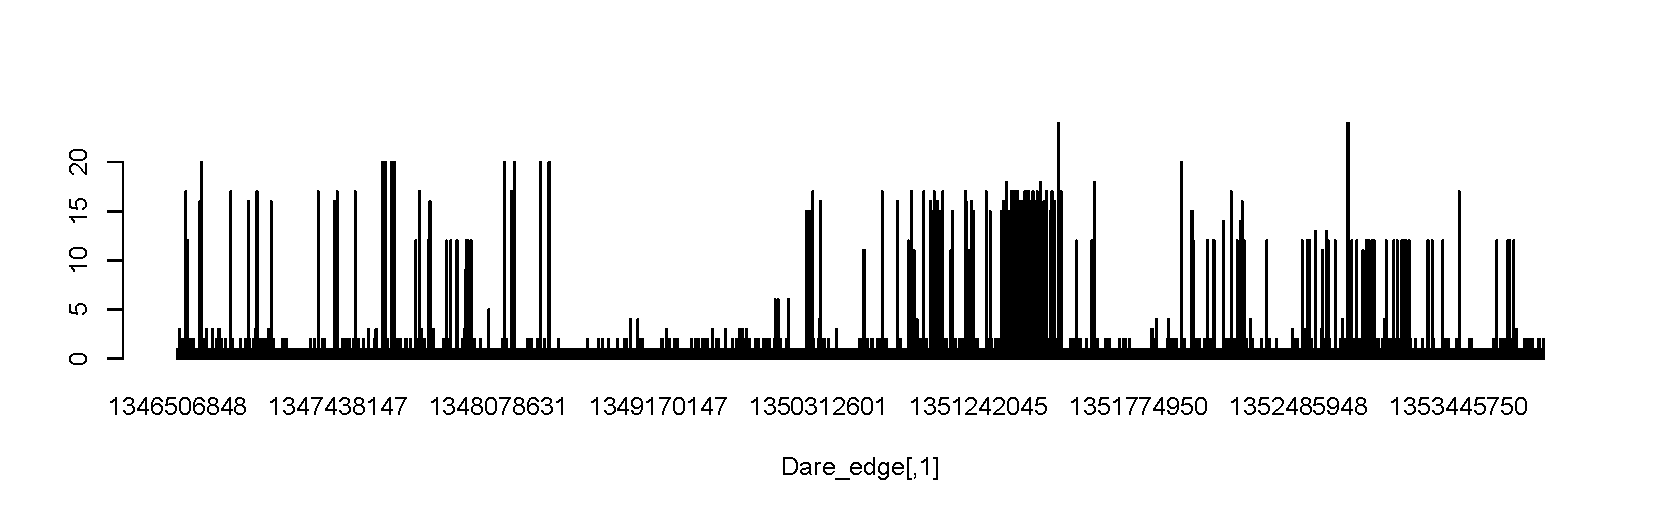
\includegraphics[width=1.1\textwidth]{DareEmails.pdf} 
	\caption{Frequency of Dare county emails from 2012-09-01 to 2012-11-30  }
	\label{fig:Emailplots}
\end{figure}
\begin{table}[ht]
	\centering
	\begin{tabular}{ |c|cc| } 
		\hline 
		\textbf{Time Interval} &\textbf{send} & \textbf{receive} \\ 	
		\hline  $[-\infty, t)$&  2.128, 2.659, 2.355, 2.919& 0.292, 0.257, 0.047, 0.110\\  $[t-30 m, t)$ &  0.262, -0.064, 0.782, 0.317 &2.087, 1.287 , 2.346, 1.870\\  $[t-2h, t-30m)$& 0.383, 0.157 , 0.024, -0.045 &0.553, 0.082, 0.794, 0.269\\ $[t-8h, t-2h)$ & 0.816, 0.054 , 0.077, 0.381 &-0.221, 0.048, 0.298, -0.012 \\ $[t-32h, t-8h)$& 0.085, 0.014,  0.228, 0.070 &0.101, 0.017, -0.033, 0.019\\ $[t-5.33d, t-32h)$&  0.103, 0.025, 0.092, 0.008 &-0.027, -0.016, -0.033, -0.009 \\ $[t-21.33d, t-5.33d)$  & 0.052, 0.000, 0.059, 0.010& 0.013, 0.030 , -0.016, 0.013\\ 
		$[-\infty, t-21.33d)$  & 0.052, 0.103, 0.027, 0.021  & 0.008, 0.000, 0.020, -0.005\\
		\hline
	\end{tabular}
	\caption {Estimated coefficients and approximate standard errors for dyadic effects of Dare county data (before Sandy, during Sandy, after Sandy, overall)}
	\label{table:nullDare}
\end{table}
\footnotesize
\begin{figure}[ht]
	\centering
	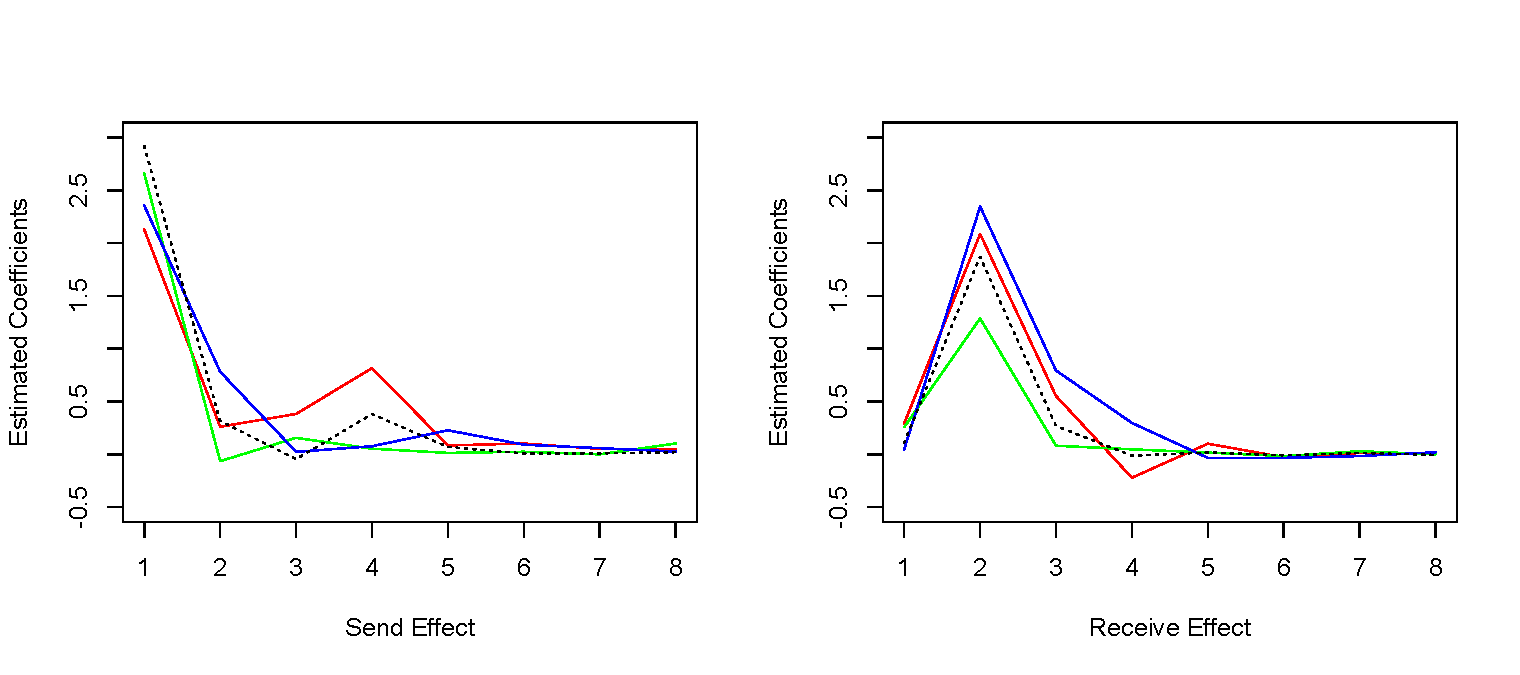
\includegraphics[width=1.1\textwidth]{Dareplot.pdf} 
	\caption{Comparison of Send (left) and Receive (right) effect based on periods in Table 1. (Red=Before, Green=During, Blue=After, and dot=Overall)}	\label{fig:Emailplo22t}
\end{figure}
\subsection{Lenoir County}
\footnotesize
\begin{table}[ht]
	\centering
	\begin{tabular}{ |c|ccc|c| } 
		\hline 
		\textbf{Period} &\textbf{Before Sandy} & \textbf{During Sandy} & \textbf{After Sandy} & \textbf{Overall} \\ 	\hline
		\textbf{\# emails}& 216 & 83 & 302 & 601 \\ 
		\hline
	\end{tabular}
	\caption{ Summary of Lenoir county email data based on time period}
	\label{table:nullDare22}
\end{table}
\normalsize
Before Sandy ranges from 2012-10-01 to 2012-10-21 (3 weeks), During Sandy ranges from 2012-10-22 to 2012-11-02 (2 weeks), and After Sandy ranges from 2012-11-03 to 2012-12-31 (8 weeks).
\footnotesize
\begin{figure}[ht]
	\centering
	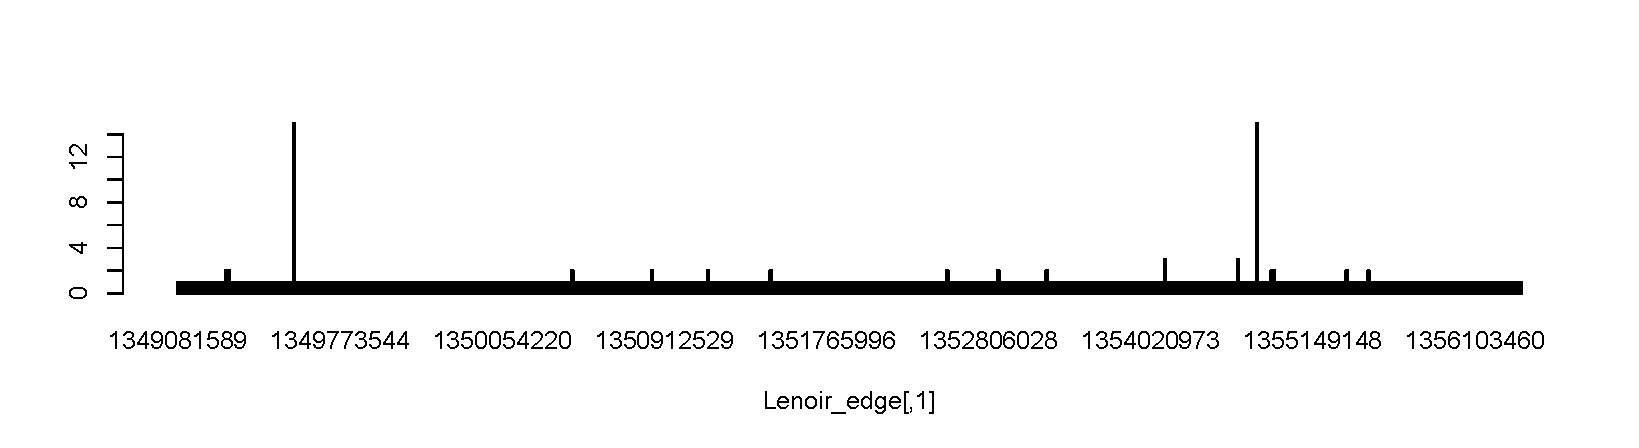
\includegraphics[width=1.1\textwidth]{LenoirEmails.pdf} 
	\caption{Frequency of Lenoir county emails from 2012-10-01 to 2012-12-31  }
	\label{fig:Emailplots32}
\end{figure}
\newpage
\subsection{Vance County}
\footnotesize
\footnotesize
\begin{table}[ht]
	\centering
	\begin{tabular}{ |c|ccc|c| } 
		\hline 
		\textbf{Period} &\textbf{Before Sandy} & \textbf{During Sandy} & \textbf{After Sandy} & \textbf{Overall} \\ 	\hline
		\textbf{\# emails}& 198& 18 & 55 & 271 \\ 
		\hline
	\end{tabular}
	\caption{ Summary of Vance county email data based on time period}
	\label{table:nullVance}
\end{table}
\normalsize
Before Sandy ranges from 2012-09-04 to 2012-10-21 (7 weeks), During Sandy ranges from 2012-10-22 to 2012-11-02 (2 weeks), and After Sandy ranges from 2012-11-03 to 2012-11-30  (4 weeks).
\footnotesize
\begin{figure}[ht]
	\centering
	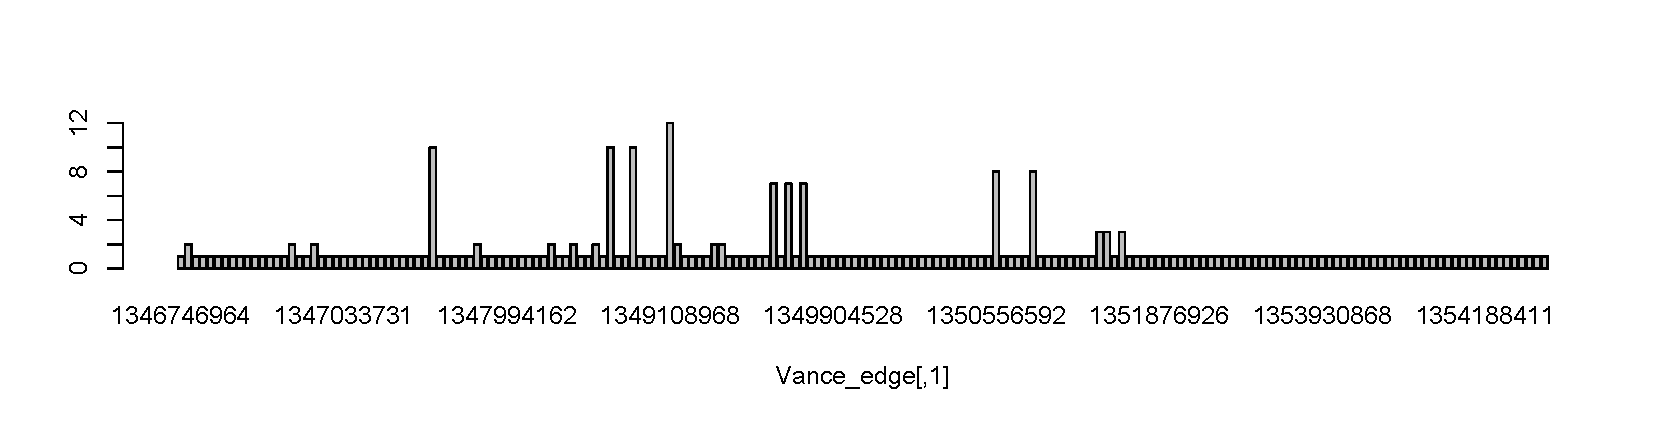
\includegraphics[width=1.1\textwidth]{VanceEmails.pdf} 
	\caption{Frequency of Vance county emails from 2012-09-04 to 2012-11-30  }
	\label{fig:Emailplots22}
\end{figure}

\bibliographystyle{apalike}
\bibliography{BominBib}

\end{document}